\documentclass[12pt]{article}
\usepackage[UTF8]{ctex}
\usepackage{geometry}
\usepackage{listings}
\usepackage{graphicx}
\usepackage{subfigure}
\usepackage{array}
\usepackage{caption}    
\usepackage{float}
\usepackage{hyperref}
\usepackage{bookmark}

\geometry{left=15mm,right=15mm,top=20mm,bottom=20mm}
\title{第二次作业报告}
\author{PB21010362 汪兆辰}
\date{\today}
\newcommand{\upcite}[1]{\textsuperscript{\textsuperscript{\cite{#1}}}}
\begin{document}
\maketitle

\section{算法介绍}
程序采用RBF算法,通过设定一系列参考点将原图im中的像素点插值计算映射到像im2中的对应位置。变换函数为
\begin{equation}
    f(x)= \Sigma_{i=1}^N a_i b_i(x)
\end{equation}
其中$b_i (x)$是径向函数,可定义为:
\begin{equation}
    b_i (x)=\frac{1}{|x-p_i|^2+d}
\end{equation}
式中N为参考点$p_i$的个数,x为原图im中点的位置,$f(x)$为像点的位置,d为参数.

将$p_i,q_i$代入可得到方程:
\begin{equation}
    Q=PA
\end{equation}
其中Q为参考点为行向量组成的N*2矩阵,P为N*N矩阵且满足$P(i,j)=\frac{1}{|p_i -q_j|^2 +d}$,A为系数$a_i$为行向量组成的
N*2矩阵.由该方程可解出系数矩阵A.

将im中的点遍历并带入$f(x)$,计算结果经四舍五入为im2中点的坐标后,就得到了im经过RBF变换后的图像.

\section{算法实现}

\subsection{使用幂函数的算法实现}

将$b_i(x)$定义如上,设置参数d=1e6,代码如下:
\begin{lstlisting}
N=size(psrc,1);
P=zeros(N);
d=1e5;
for i=1:1:N
    for j=1:1:N
        p=psrc(i,:);
        q=pdst(j,:);
        P(i,j)=1/(norm(p-q)^2+d);
    end
end
A=P\(pdst-psrc);
for i=1:h
    for j=1:w
        for k=1:dim
            x=[j,i];
            fx = zeros(1,2);
            for m = 1:N
                fx = fx+A(m,:)/(norm(x-psrc(m,:))^2+d);
            end
            fx=fx+x;
            if fx(1,1)>0&&ceil(fx(1,1))<=h&&fx(1,2)>0&&ceil(fx(1,2))<=w
                im2(ceil(fx(1,2)),ceil(fx(1,1)),k)=im(i,j,k);
            else
            end
        end
    end
end
\end{lstlisting}

图像处理的结果如下:
\begin{figure}[H]
    \centering
    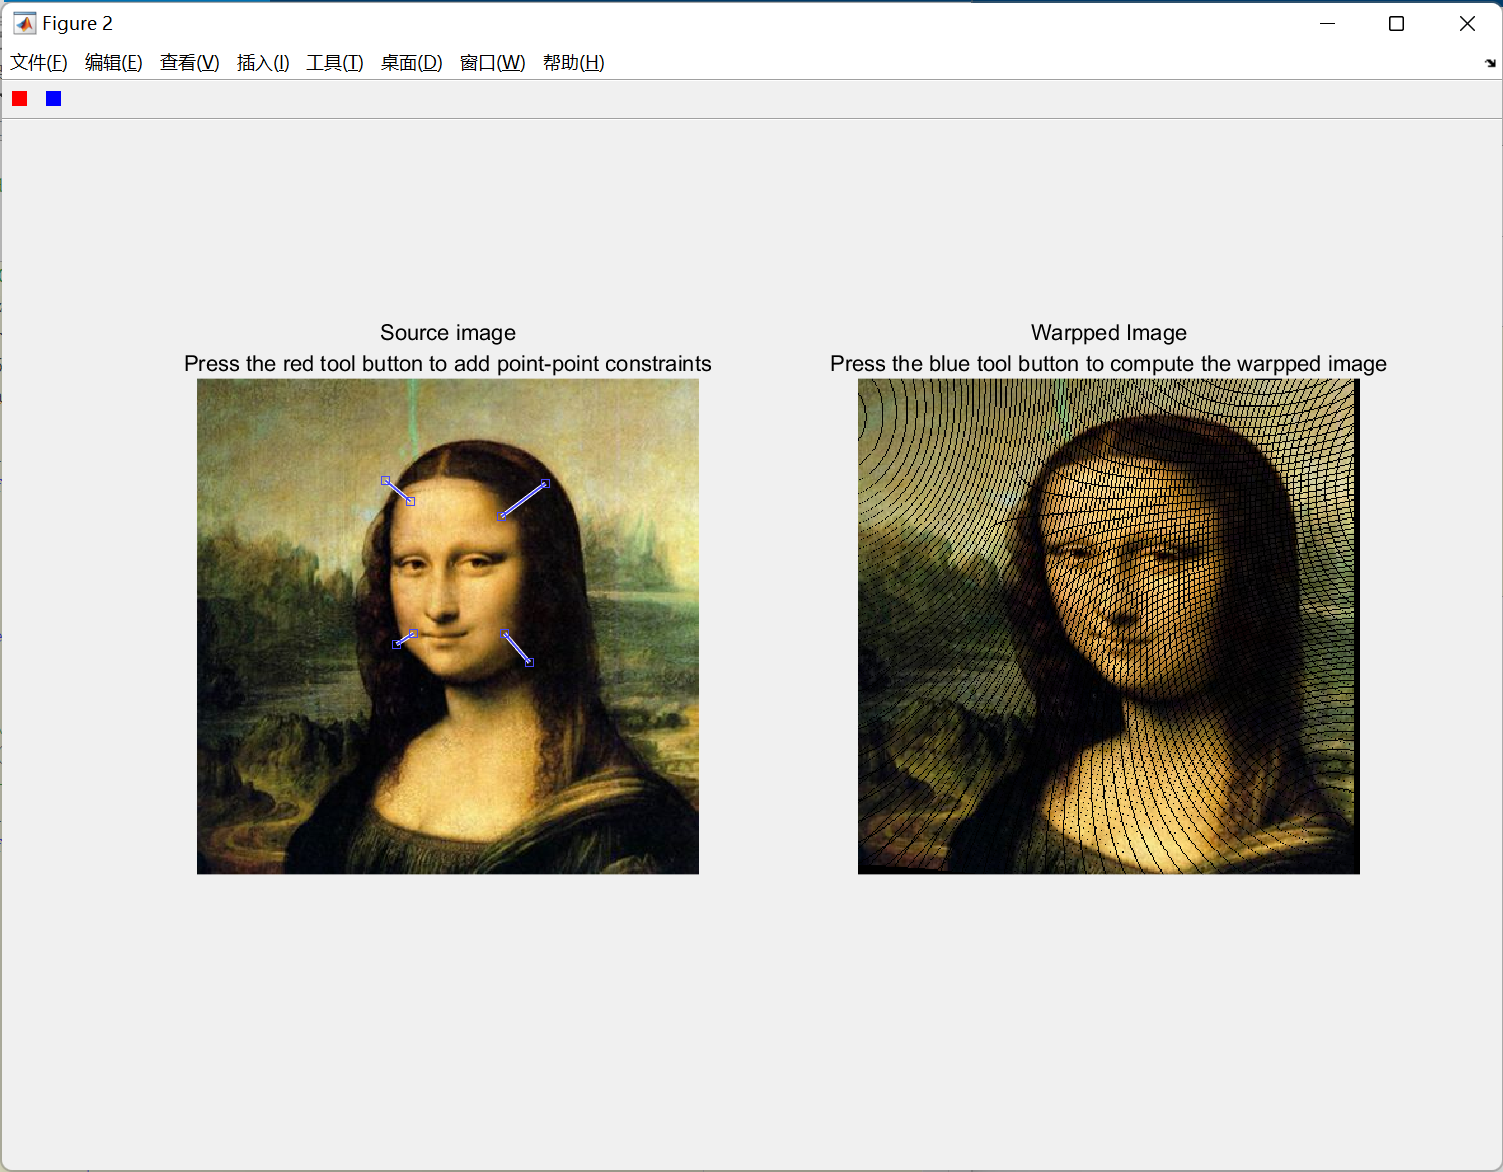
\includegraphics[scale=0.4]{pic1.png}
\end{figure}

注意到此变换不保持局部性,即整张图都因变换产生较大变化,与预期只有参考点附近变化较大不符,因而考虑采用高斯函数来替代幂函数.

\subsection{使用高斯函数的算法实现}
高斯函数的形式为:
\begin{equation}
    g(t)=e^{-t^2 / \delta ^2}
\end{equation}
可以证明\upcite{1},利用高斯函数可以使得离参考点较远的点经变换后还在原位置附近,而离参考点较远的点经变换会发生较大变化.

代码只需将上述代码的$b_i (x)$修改成高斯函数$g_i (x)$,不再展示修改后的代码.

取$\delta ^2 =2200$, 图像处理的结果如下:
\begin{figure}[H]
    \centering
    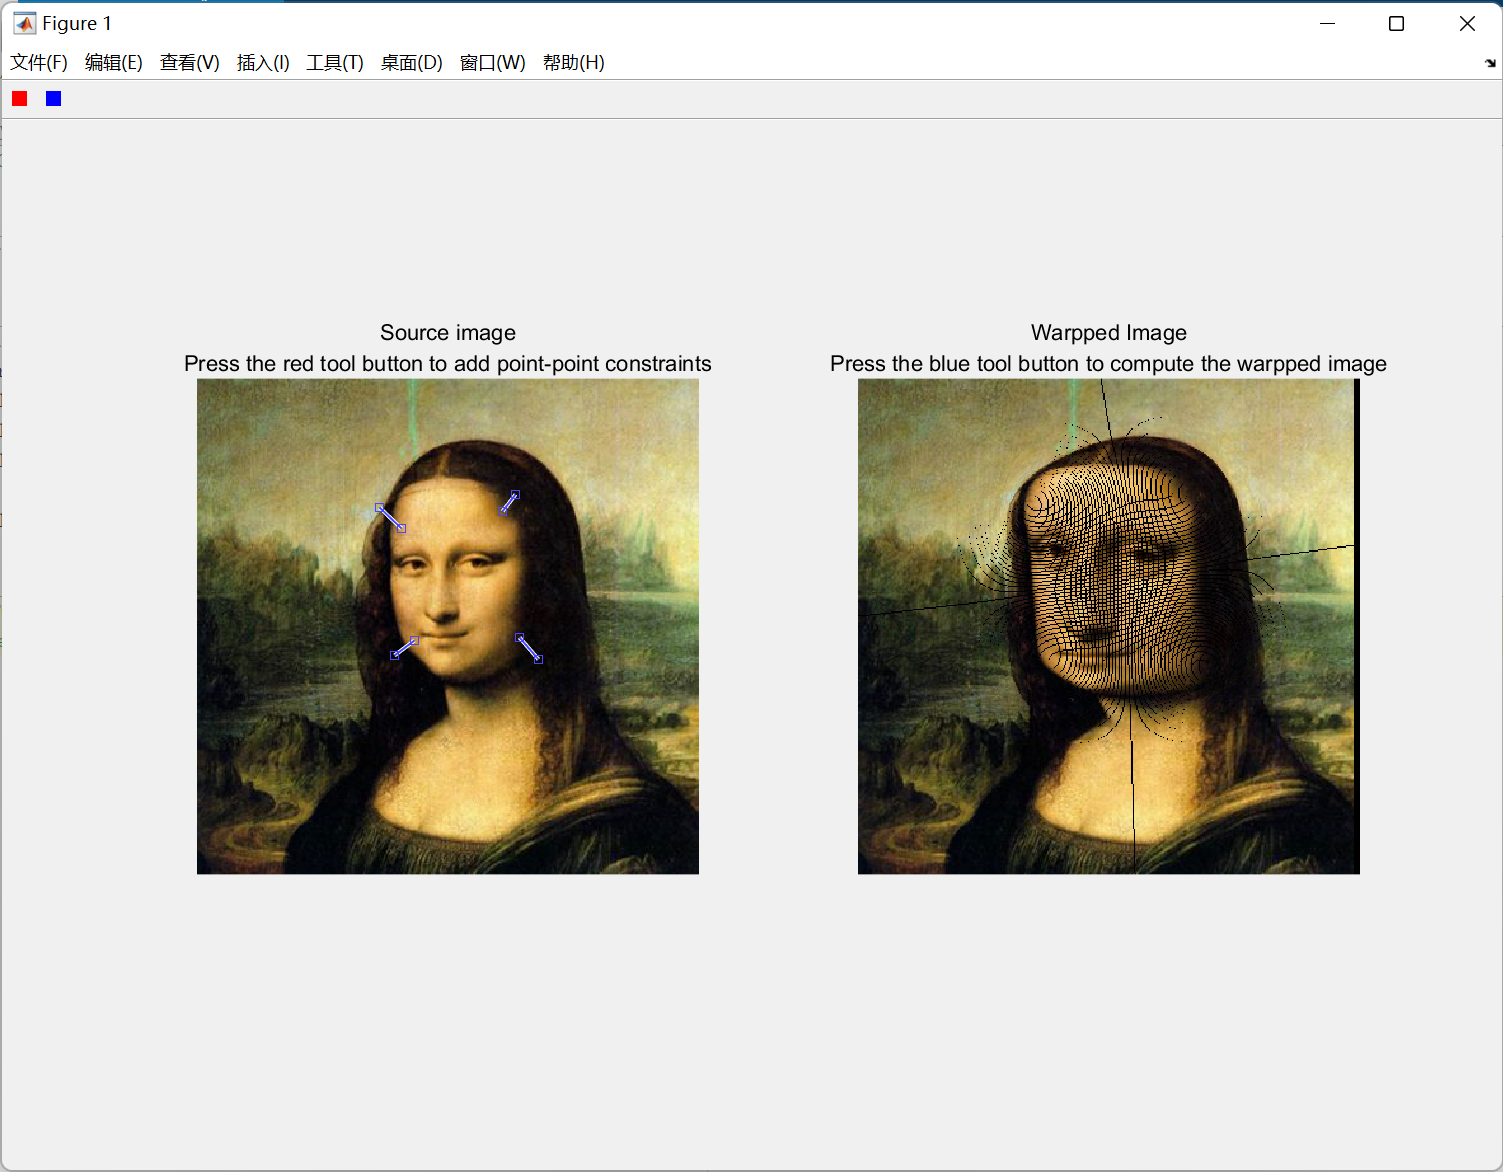
\includegraphics[scale=0.4]{pic2.png}
\end{figure}

\section{算法的进一步完善}

容易发现按照上述算法进行图像处理后图像中有大量黑色条纹,这是由于一方面源图像的存储结构为对像素点进行采样后得到的矩阵,本身已经是离散的,经过RBF变换后更无法保证像的每个像素点连续;另一方面
由于计算得到的坐标并非整数,在赋值过程中经过了取整,导致条纹处的点没有原像.因此需要在已有算法基础上进一步完善.

\subsection{尝试使用卷积}
卷积可以使图像模糊或“平滑”,于是尝试用卷积解决上述问题,代码如下:
\begin{lstlisting}
% Create Gauss filter
kernel_size = 5;
sigma = 2;
gauss_kernel = fspecial('gaussian', [kernel_size kernel_size], sigma);

% convolution
im2(:,:,1) = conv2(im2(:,:,1), gauss_kernel, 'same');
im2(:,:,2) = conv2(im2(:,:,2), gauss_kernel, 'same');
im2(:,:,3) = conv2(im2(:,:,3), gauss_kernel, 'same');
\end{lstlisting}
图像处理的结果如下:
\begin{figure}[H]
    \centering
    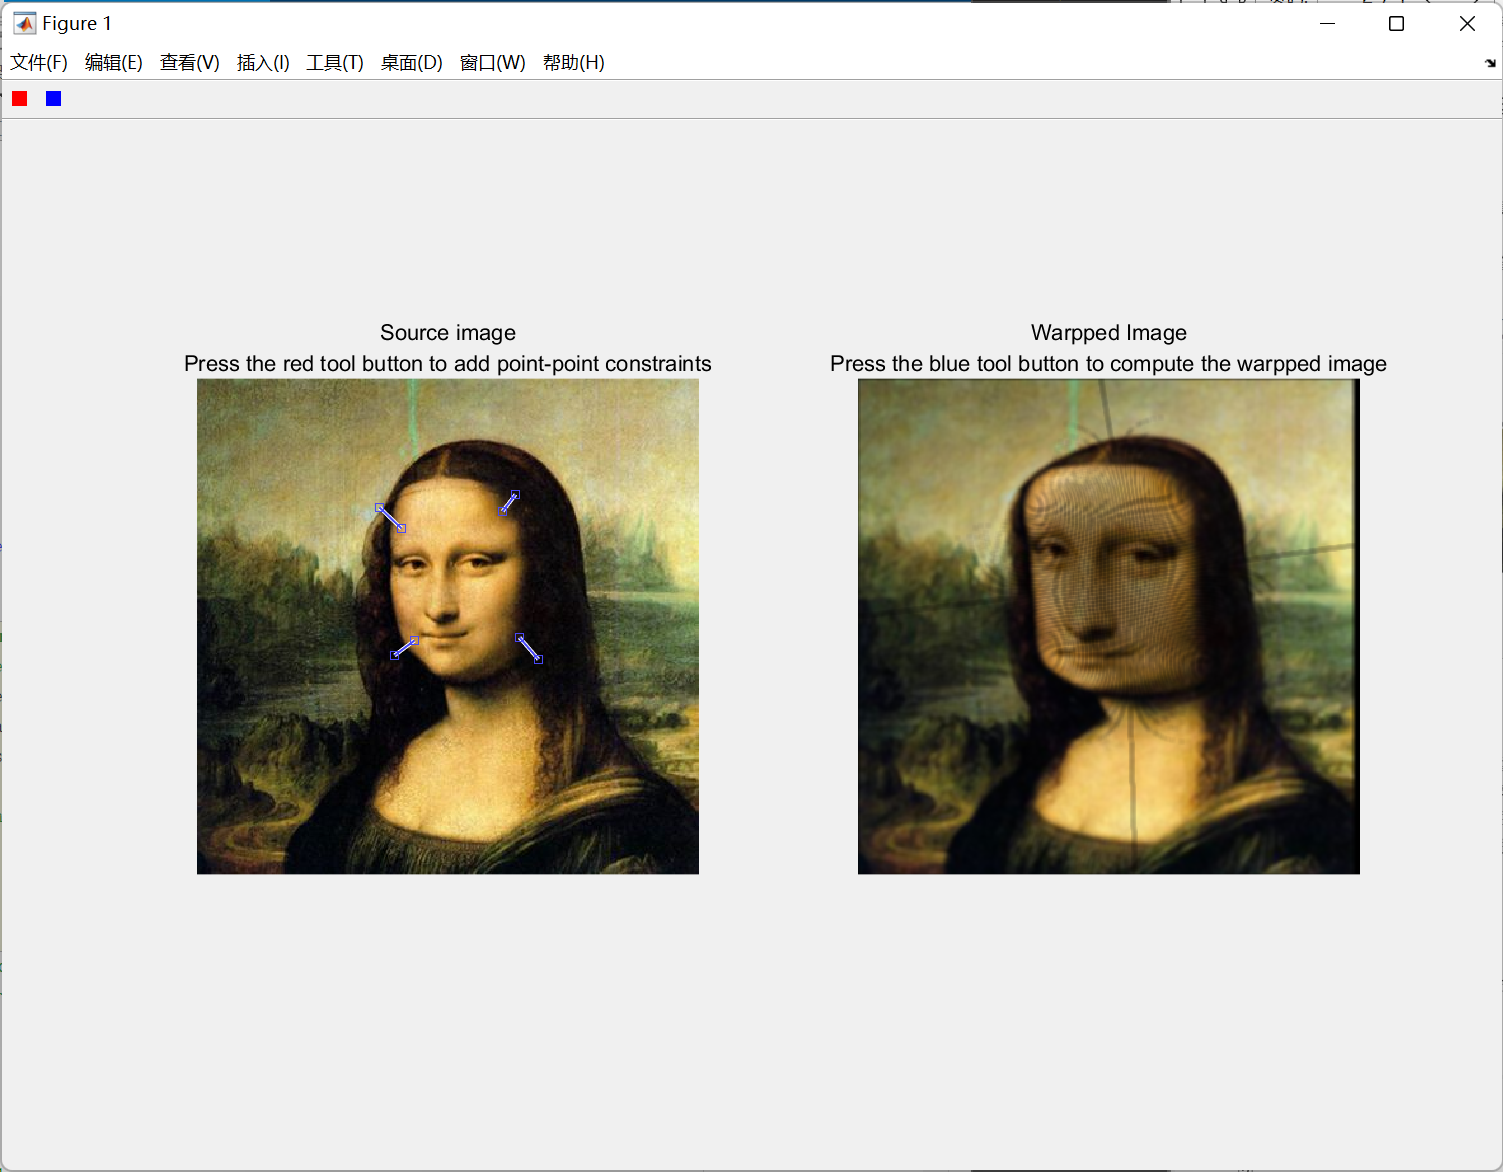
\includegraphics[scale=0.4]{pic3.png}
\end{figure}
发现卷积并未完全消除黑色条纹,反而由于卷积的平均作用,整张脸的颜色都明显变暗,处理效果并不理想.而且这也只是对图像的二次处理,并不解决本质问题,需要寻找其他的解决方案.

\subsection{尝试使用逆变换}
RBF算法的变换是将所有im中的点经过变换找到im2上的点与之对应,则黑色条纹中的点也应该可以对应回im中的某个点,而且应该是多个im2中的点都对应到im上一个点.按照这种思想,我们只需要解非线性方程:
\begin{equation}
    y=\Sigma _{i=1}^N a_i b_i(x)
\end{equation}
其中y取遍im2中点的坐标.代码如下:
\begin{lstlisting}
for t=1:N
    sum=sum+A(t,:)/(norm(x-psrc(t,:))^2+d);
end
F=@(x) sum+x-[i,j];
solution=fzero(F,[1,1]);
\end{lstlisting}
fzero用数值逼近方程的解,但该方法的计算量过大,还应寻找更好的算法.

\subsection{一种形式上的“反变换”}
原算法出现黑色条纹的一部分原因是因为变换并非满射,为了消除结果的条纹,我们考虑从im2出发的一个单射.但在3.2中我们已经说明了
直接求得变换的反变换并不容易,甚至无法求出,于是我们转而考虑一种形式上的“反变换”.

假设原变换的效果是使图像向外“膨胀”,那么“反变换”的效果应该使图像向内“收缩”,反之亦反.那么我们只需要当RBF作用在im2时可以得到源图像im,并在处理时对p,q进行调换,
就可以得到具有“反变换”效果的一个变换,即若有原变换为:
\begin{equation}
    y=x+g(x)
\end{equation}
那么只需:
\begin{equation}
    x=y+g'(y)
\end{equation}
其中x,y分别为im,im2中的点.
图形处理的结果如下:
\begin{figure}[H]
    \centering
    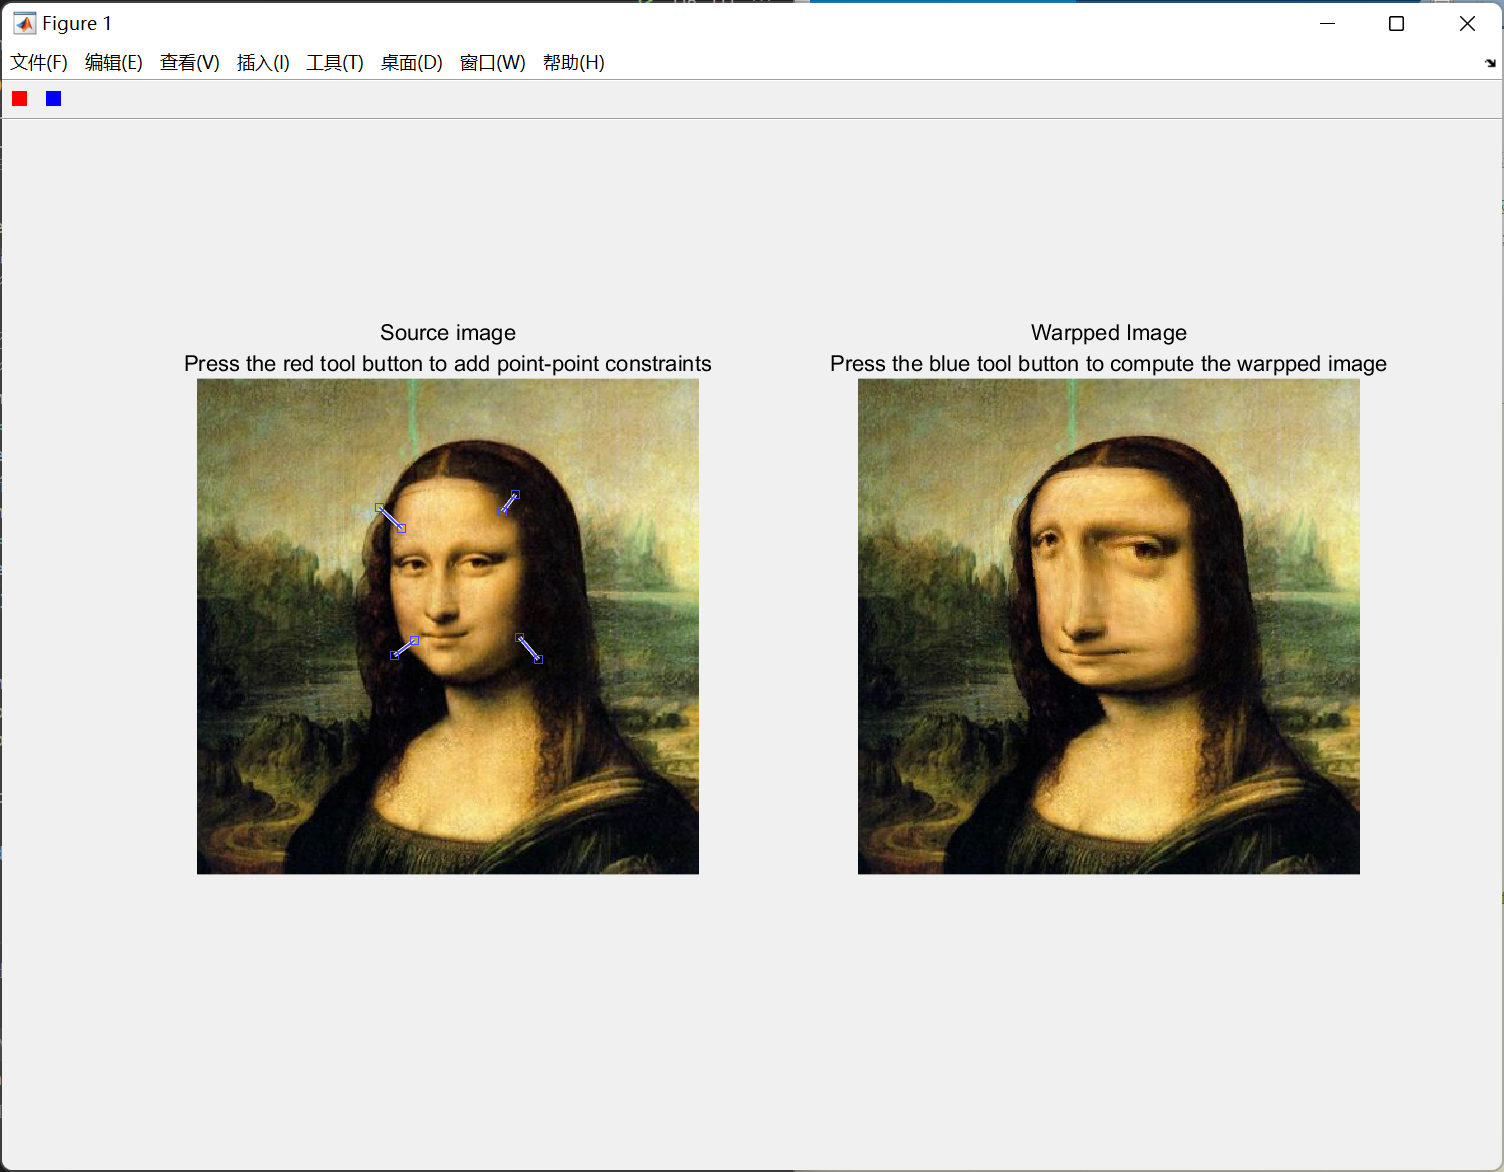
\includegraphics[scale=0.4]{pic4.png}
\end{figure}
注意这种变换并不是严格意义上的反变换,得到的图形与用之前算法得到的图形之间有差别,用这种变换直接作用在变换后的图像上也无法还原成源图像.

\begin{thebibliography}{3}
    \bibitem{1} Nur Arad and Daniel Reisfeld, Image Warping Using Few Anchor Points and Radial Functions. Computer Graphics Forum, 1995.
    \bibitem{2} \url{https://zhuanlan.zhihu.com/p/366929278}
    \bibitem{3} \url{https://blog.csdn.net/weixin_39702639/article/details/111203275}

\end{thebibliography}

\end{document}
